% Ocean Engineering submission skeleton — v2 draft content wired from
% docs/DRAFT_main_paper_v0.md (2026-07-06). Numbers verified by
% scripts/d3_final_verification.py (31/31).
\documentclass[review]{elsarticle}

\usepackage{amsmath,amssymb,amsfonts}
\usepackage{graphicx}
\usepackage{booktabs}
\usepackage{multirow}
\usepackage{hyperref}
\usepackage{xcolor}
\usepackage{subcaption}
\usepackage{lineno}

\journal{Ocean Engineering}

\begin{document}
\begin{frontmatter}

\title{Control-compatible real-time wave encounter forecasting with a
given forward-looking LiDAR: information limits, streaming
equivalence, and self-diagnosed reliability}

% \author[inst1]{...}
% \affiliation[inst1]{...}

\begin{abstract}
% docs/DRAFT_main_paper_v0.md Abstract — paste at v2-final
Wave-preview feedforward control of fast foiling vessels requires a
phase-resolved forecast of the encountered surface elevation within a
hard real-time budget. We ask what a \emph{given} commercial
forward-looking LiDAR can deliver on a \emph{given} vessel (a foiling
hydrofoil at 22\,kt), and whether the system can know, online, when
its forecast is trustworthy. [FULL ABSTRACT: see markdown draft.]
\end{abstract}

\begin{keyword}
wave prediction \sep deterministic sea wave prediction \sep LiDAR \sep
hydrofoil \sep predictable zone \sep recursive estimation \sep
reliability
\end{keyword}

\end{frontmatter}
% \linenumbers

\section{Introduction}\label{sec:intro}
% markdown §1 (완문) — paste & cite-wire

\section{Problem setting and information analysis}\label{sec:info}
% markdown §2 (완문): 2.1 observation class / 2.2 predictable zone
% (Fig.~\ref{fig:horizon}) / 2.3 limit ladder (Table~\ref{tab:ladder})
% / 2.4 slope ceiling

\begin{figure}[t]\centering
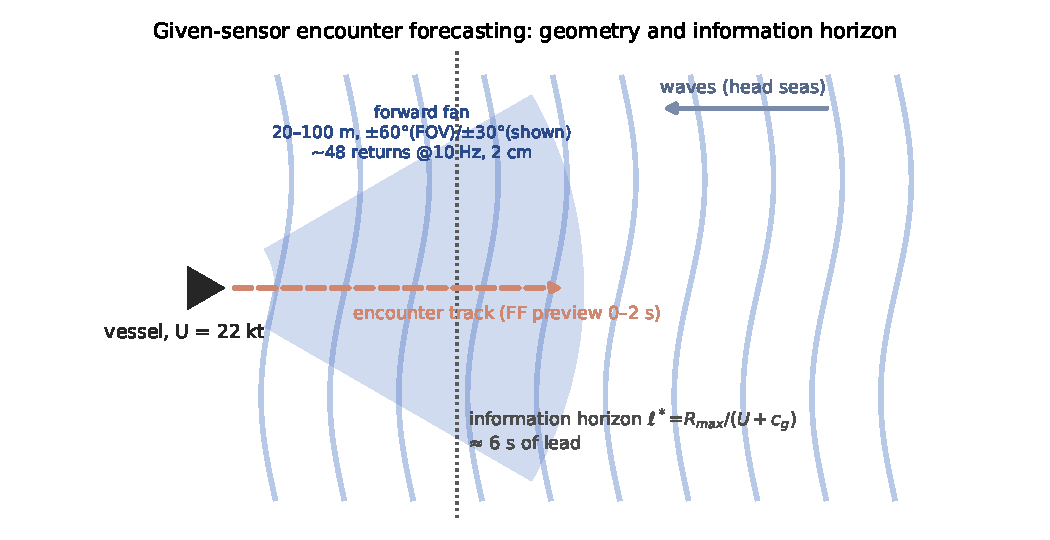
\includegraphics[width=.85\linewidth]{figures/fig_concept.pdf}
\caption{Geometry and information horizon of given-sensor encounter
forecasting.}\label{fig:concept}
\end{figure}

\begin{figure}[t]\centering
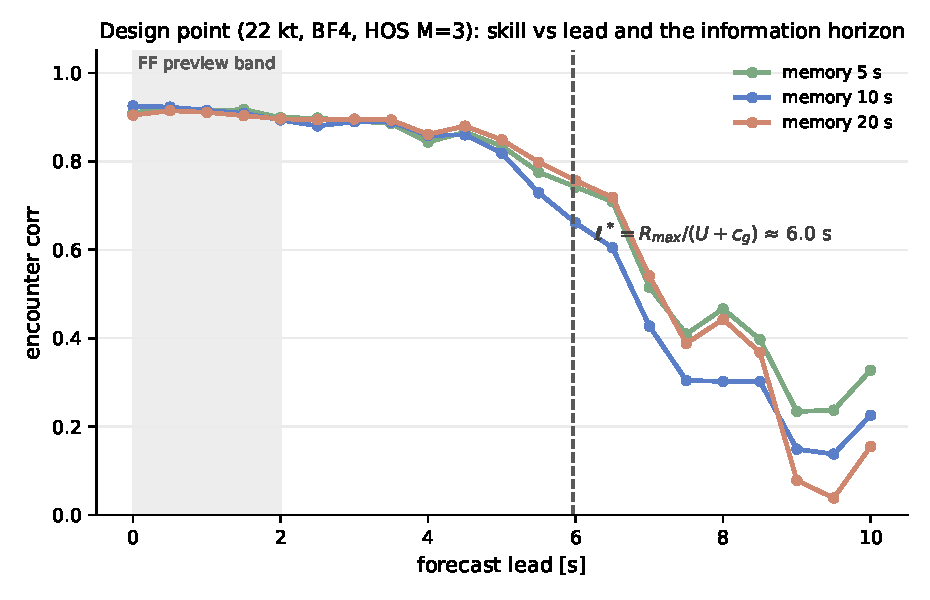
\includegraphics[width=.9\linewidth]{figures/fig_horizon.pdf}
\caption{Design point (22\,kt, BF4, HOS M=3, $n{=}12$ seas): encounter
skill vs.\ lead and the predicted horizon
$\ell^*\!=\!R_{max}/(U{+}c_g)$.}\label{fig:horizon}
\end{figure}

\section{A streaming estimator that attains the limit}\label{sec:stream}
% markdown §3 (완문): bank MMSE / RLS equivalence (derivation box) /
% two-timescale / measured latency; Table CN-RLS 대비

\section{Validation}\label{sec:valid}
% markdown §4: three legs; Fig.~\ref{fig:robust}; Fig.~\ref{fig:sites}

\begin{figure}[t]\centering
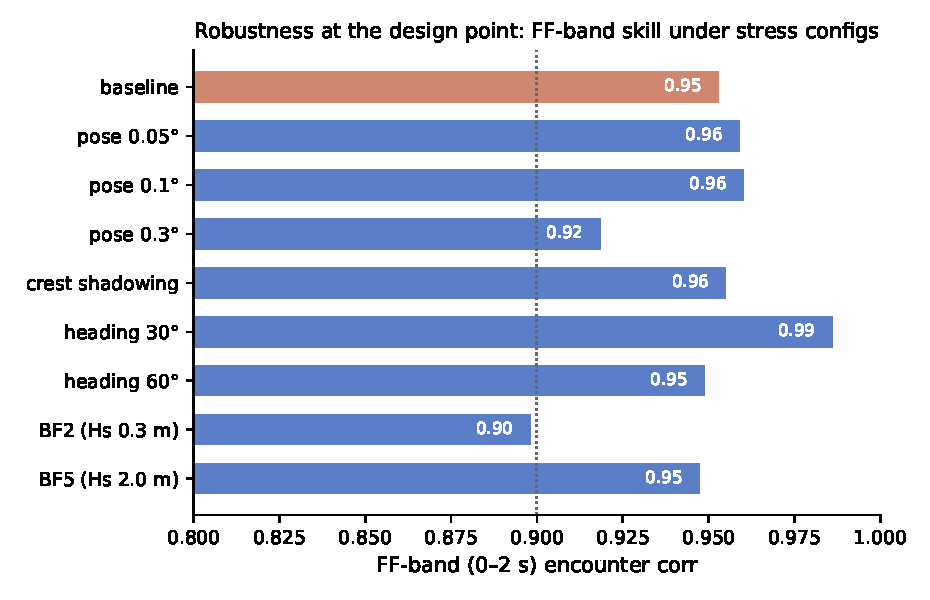
\includegraphics[width=.9\linewidth]{figures/fig_robust.pdf}
\caption{Robustness of FF-band skill at the design point.}
\label{fig:robust}
\end{figure}

\begin{figure}[t]\centering
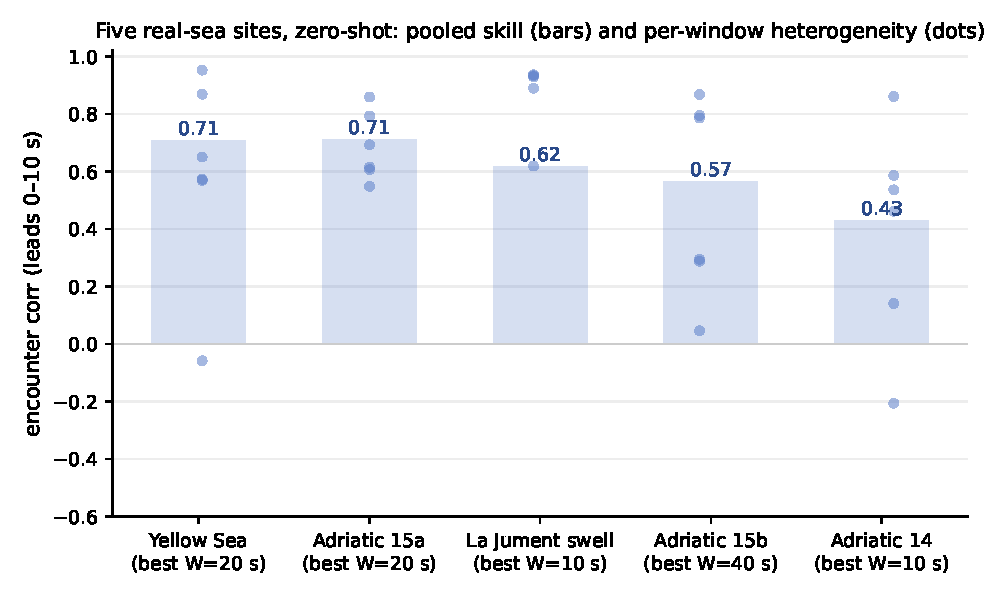
\includegraphics[width=.9\linewidth]{figures/fig_sites.pdf}
\caption{Five real-sea sites, zero-shot: pooled skill and per-window
heterogeneity.}\label{fig:sites}
\end{figure}

\section{Real-sea failure forensics and a preliminary reliability
gate}\label{sec:gate}
% markdown §5 incl. pre-registered confirmations (exploratory vs
% confirmatory labels); Fig.~\ref{fig:gate}

\begin{figure}[t]\centering
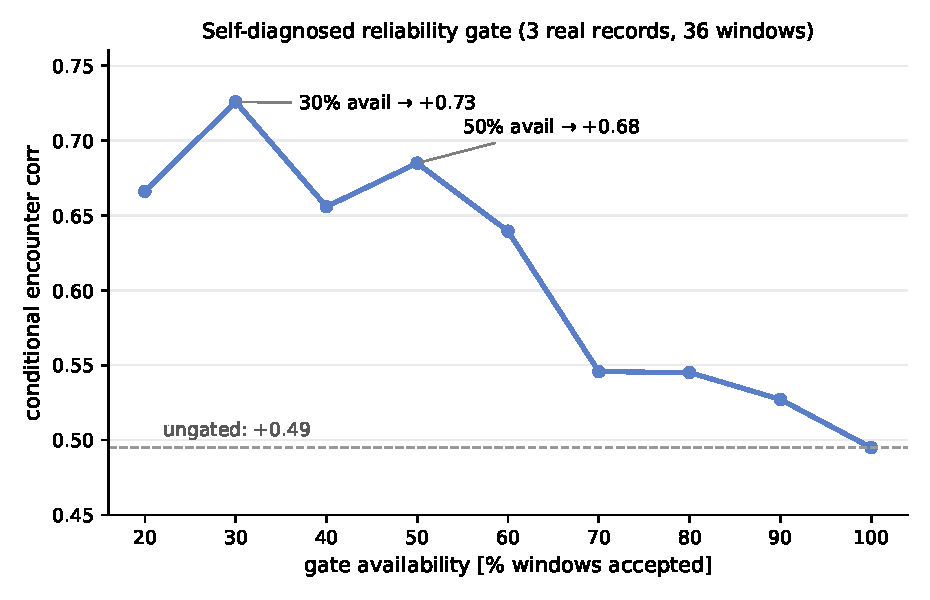
\includegraphics[width=.8\linewidth]{figures/fig_gate_roc.pdf}
\caption{Site-adaptive residual gate: reliability vs.\ availability
(exploratory; confirmations reproduce direction, not significance).}
\label{fig:gate}
\end{figure}

\section{Control closure}\label{sec:control}
% markdown §6; Fig.~\ref{fig:e2e}

\begin{figure}[t]\centering
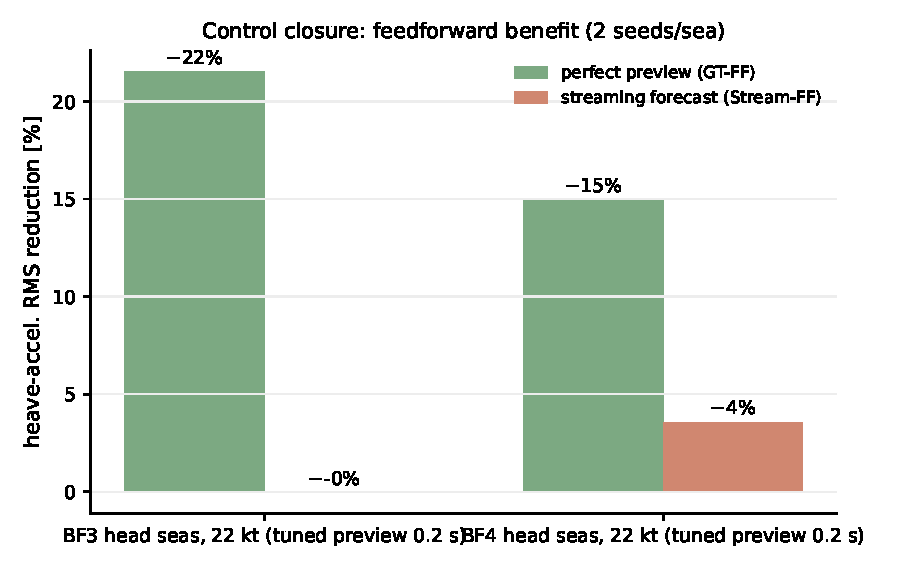
\includegraphics[width=.75\linewidth]{figures/fig_e2e.pdf}
\caption{Feedforward benefit with the tuned controller.}\label{fig:e2e}
\end{figure}

\section{Limitations and requirements for the next tier}\label{sec:lim}
% markdown §7

\section{Conclusions}\label{sec:concl}
% markdown §8 (완문)

\section*{Data and code availability}
Validation uses the open stereo dataset of Guimar\~aes et al.\ (2020),
CC BY 4.0, IFREMER SEXTANT
(doi:10.12770/af599f42-2770-4d6d-8209-13f40e2c292f). All headline
numbers re-derive from released result files via a single verification
script (31/31).

% \bibliographystyle{elsarticle-num}
% \bibliography{references}
\end{document}
